%%%%%%%%%%%%%%%%%%%%%%%%%%%%%%%%%%%%%%%%%%%%%%%%%%%%%%%%%%%%%%%%%%
\section{Leaflet driven by a sinusoidal channel flow}
\label{sec:leaflet}
%%%%%%%%%%%%%%%%%%%%%%%%%%%%%%%%%%%%%%%%%%%%%%%%%%%%%%%%%%%%%%%%%%

The second benchmark exercises the coupling under strong time-dependent forcing. A thin flexible leaflet, clamped along one edge, oscillates in response to a periodic channel flow whose direction reverses every half-period. The configuration is taken from the immersed finite element method (IFEM) study of \citet{zhang_immersed_2007}, where it serves as the canonical FSI verification case, and it has since been used by several groups developing related immersed and fictitious-domain formulations \citep{baaijens_fictitiousdomain_2001,de_hart_threedimensional_2003,zhang_immersed_2012,roy_benchmarking_2015}. Although the geometry is deliberately idealised, it isolates a regime representative of physiological heart-valve dynamics, and the combination of strong unsteady forcing, large structural rotation, and bidirectional loading makes it a stringent test of whether an FSI scheme transfers momentum and kinematic information consistently across the interface.

In the original study the leaflet is modelled as a two-dimensional nearly incompressible hyperelastic continuum discretised by quadrilateral finite elements and immersed in a non-conforming Eulerian finite element fluid mesh. Coupling is established through a smoothed Dirac-delta-like interpolation operator borrowed from the reproducing kernel particle method, which both spreads the interaction forces from the solid to the fluid and interpolates the fluid velocity onto the solid. The formulation generalises Peskin's immersed boundary method \citep{peskin_immersed_2002} by removing the assumption of a fibre-like solid and relaxing the requirement of a uniform background mesh, and the leaflet is anchored by tethering its clamped edge to a fixed material point through a stiff penalty force \citep{de_hart_threedimensional_2003}. The leaflet response is fully resolved as a two-dimensional continuum, including through-thickness stretching and shearing and the surrounding tractions on its faces. The present approach instead reduces the structure to a slender Simo--Reissner beam whose centreline coincides with the leaflet mid-line, with the rectangular cross-section entering only through its inertia and bending stiffness, and couples it through the actuator-line operators of Section~\ref{sec:almCouplingTheory}. The leaflet therefore exerts a force on the fluid without occupying a discrete volume in the CFD mesh, and the channel mesh remains static. The framework is computationally lighter, but it introduces the modelling assumption that the leaflet is loaded by quasi-steady normal drag rather than by resolved surface tractions. Whether that assumption holds in the oscillatory low-Reynolds regime is what the benchmark assesses.

\subsection{Problem definition}
\label{sec:leaflet_geometry}
The geometry is presented in Figure~\ref{fig:leaflet_schematic} and follows \citet{zhang_immersed_2007}, Section~3.2. The fluid domain is a rectangular channel of length $L = 4~\mathrm{cm}$ and full width $2H = 2~\mathrm{cm}$, with the origin where the inlet plane meets the channel mid-plane. The leaflet is a thin flexible body of length $\lambda = 0.8~\mathrm{cm}$ and thickness $t_{\ell} = 0.0212~\mathrm{cm}$, where the subscript distinguishes it from the time $t$, clamped at the mid-length of the channel and free at the other end. Because the clamped end is anchored on the channel mid-plane, the leaflet is symmetric about the line that bisects the channel along its length, and only one half of the original domain is simulated. The mid-plane is treated as a symmetry boundary on which the leaflet root resides, so the simulated transverse extent is $H = 1~\mathrm{cm}$. The domain depth in the third direction equals $t_{\ell}$ with symmetry conditions on the two transverse faces, so the simulation remains effectively two-dimensional while retaining the leaflet thickness in the projection operators.

\begin{figure}[!ht]
\centering
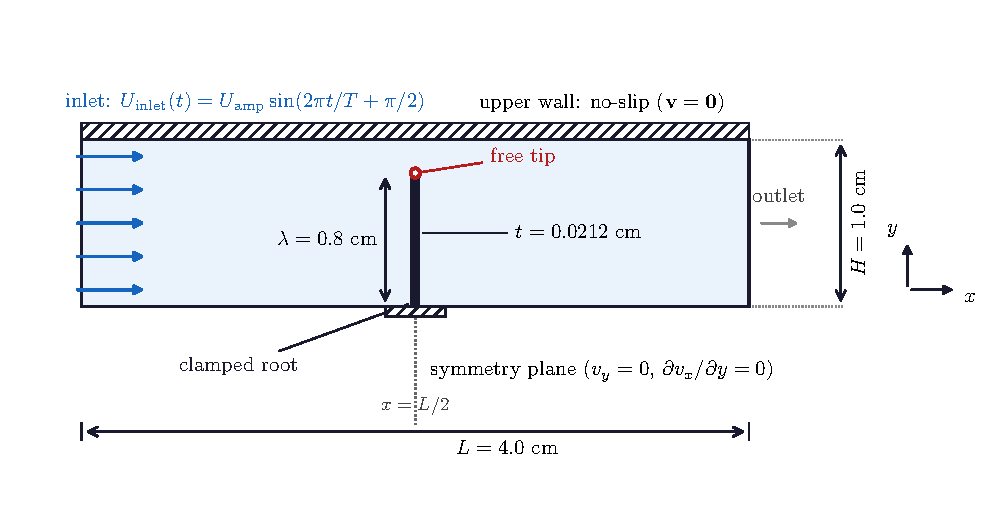
\includegraphics[width=0.88\textwidth]{leaflet_schematic.pdf}
\caption{The leaflet-in-channel verification problem, drawn as the simulated half-domain. The leaflet, of length $\lambda$ and thickness $t_{\ell}$, is clamped at the channel mid-plane at $x = L/2$ and free at its tip. A sinusoidal channel flow is imposed at the inlet, the opposite wall is no-slip, and the lower edge is a symmetry boundary. Dimensions reproduce \citet{zhang_immersed_2007}, Section~3.2.}
\label{fig:leaflet_schematic}
\end{figure}

A spatially uniform, time-periodic horizontal velocity is prescribed at the inlet,
\begin{equation}
U_{\mathrm{inlet}}(t) = U_{\mathrm{amp}} \sin\!\left(\frac{2\pi t}{T} + \frac{\pi}{2}\right),
\label{eq:leaflet_inlet}
\end{equation}
so the flow begins at its peak amplitude, the phase shift being chosen for consistency with the original paper in which the leaflet is released from rest into a fully developed inflow. The downstream boundary is a zero-gradient outflow with a fixed reference pressure, the upper boundary a stationary no-slip wall, and the lower boundary a symmetry plane that simultaneously models the channel mid-plane and anchors the leaflet root. Both the fluid and the leaflet start at rest with the leaflet undeformed.

The fluid is a Newtonian incompressible liquid of density $10^{3}~\mathrm{kg\,m^{-3}}$, and the leaflet has density $\rho_{s} = 6\times10^{3}~\mathrm{kg\,m^{-3}}$, Young's modulus $E = 10^{6}~\mathrm{Pa}$, and Poisson ratio $\nu = 0.5$. In the IFEM reference the Poisson ratio enters explicitly through the hyperelastic strain-energy function of a nearly incompressible continuum, whereas in the present beam formulation only the shear modulus $G = E/[2(1+\nu)]$ is used, evaluated at the same reference value for consistency with the original constitutive description. The regime is characterised by a Reynolds number $\mathrm{Re} = \rho\,U_{\mathrm{amp}}\,H / \mu$ and a Strouhal number $\mathrm{St} = H / (U_{\mathrm{amp}}\,T)$, defined as in the reference paper. The four combinations used here are listed in Table~\ref{tab:leaflet_cases}.

\begin{table}[!ht]
\centering
\small
\caption{Forcing parameters for the four (Re, St) cases of \citet{zhang_immersed_2007}, Section~3.2, with the cross-section Reynolds and Keulegan--Carpenter numbers $\mathrm{Re}_{t} = \rho\,U_{\mathrm{amp}}\,t_{\ell}/\mu$ and $\mathrm{KC} = U_{\mathrm{amp}}\,T/t_{\ell}$. All cases share $\rho = 10^{3}~\mathrm{kg\,m^{-3}}$, $H = 10^{-2}~\mathrm{m}$, and $t_{\ell} = 2.12\times10^{-4}~\mathrm{m}$. The last column is the normal drag coefficient passed to the closure, taken from the rigid-plate channel calibration of Section~\ref{sec:leaflet_cd_calibration} at each case's own Reynolds number.}
\label{tab:leaflet_cases}
\setlength{\tabcolsep}{6pt}
\renewcommand{\arraystretch}{1.15}
\begin{tabular}{c c c c c c c c}
\toprule
Case & $U_{\mathrm{amp}}$ (m\,s$^{-1}$) & $T$ (s) & $\mu$ (Pa\,s) & $\mathrm{Re}$ & $\mathrm{St}$ & $\mathrm{KC}$ & $C_{dn}$ \\
\midrule
C1 & $0.01$ & $1$ & $10^{-2}$ & $10$ & $1.0$ & $47$ & $108$ \\
C2 & $0.01$ & $1$ & $10^{-1}$ & $1$  & $1.0$ & $47$ & $332$ \\
C3 & $0.01$ & $2$ & $10^{-1}$ & $1$  & $0.5$ & $94$ & $332$ \\
C4 & $0.01$ & $2$ & $10^{-2}$ & $10$ & $0.5$ & $94$ & $108$ \\
\bottomrule
\end{tabular}
\end{table}

\subsection{Steady-CFD calibration of the normal drag coefficient}
\label{sec:leaflet_cd_calibration}

As in Section~\ref{sec:beamtunnel_cd_calibration}, $C_{dn}$ must reflect the drag that would act on a rigid leaflet of the same cross-section in the same channel at the same Reynolds number. Two steady-CFD setups are used, illustrated in Figure~\ref{fig:leaflet_dragCalib_mesh}. The first is an unbounded cross-section calibration, which measures the free-stream drag $C_{d}^{\infty}$ of the leaflet cross-section in isolation. The second is a rigid-plate channel calibration, which measures the in-channel drag $C_{d}$ of the full leaflet in the coupled domain. Both are solved with \texttt{simpleFoam} on \texttt{snappyHexMesh} grids with a level-3 refinement zone enveloping the plate and level-$(4,5)$ surface refinement on the plate itself, giving a smallest cell at the plate of $1.3\times10^{-5}~\mathrm{m}$ and $8\times10^{-6}~\mathrm{m}$ respectively. The channel calibration uses the same $150\times38$ background mesh as the coupled simulation, which removes any mesh-related component of the discrepancy between the calibration result and the value seen by the closure at run time.

\begin{figure}[!ht]
\centering
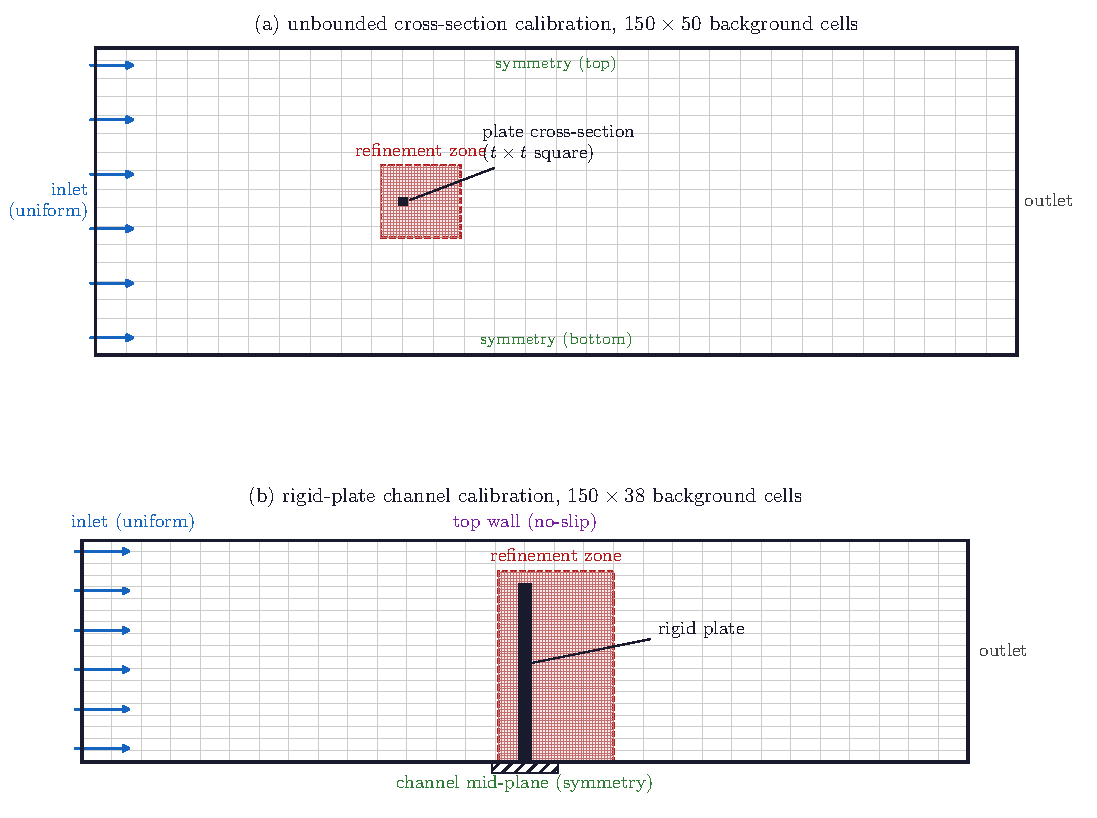
\includegraphics[width=0.88\textwidth]{leaflet_dragCalib_mesh.pdf}
\caption{The two steady-CFD drag-calibration setups. (a) Unbounded cross-section, with the square cross-section of side $t_{\ell}$ in an unbounded stream and symmetry on all four side faces, returning the free-stream drag ($A_{\mathrm{ref}} = t_{\ell}^{2}$). (b) Rigid-plate channel, with a rigid plate of length $\lambda$ and thickness $t_{\ell}$ in the coupled channel, the mid-plane treated as a symmetry plane and the opposite wall as no-slip, returning the in-channel drag ($A_{\mathrm{ref}} = t_{\ell}\,\lambda$). A local refinement zone is shown in red.}
\label{fig:leaflet_dragCalib_mesh}
\end{figure}

In the unbounded configuration all four side faces are symmetry planes, so the case is two-dimensional-equivalent and the cross-section behaves as an infinitely long cylinder. Figure~\ref{fig:leaflet_dragCalib}(a) shows the trace decreasing monotonically to $C_{d}^{\infty} \approx 36.8$ at the C1 cross-section Reynolds number $\mathrm{Re}_{t} = 0.212$, between the Oseen estimate \citep{lamb_hydrodynamics_1932} for a low-Reynolds two-dimensional cylinder ($\approx 25$) and the empirical estimate of \citet{hoerner_fluid_1965} for a flat-plate cross-section ($\approx 50$). This is not the coefficient that should be passed to the closure, because the actual leaflet sits in a channel of half-width $H = 10\,t_{\ell}$ where the blockage and the surrounding walls modify the drag. Its role is restricted to providing a literature-comparable check on the cross-section drag and a baseline against which the confinement amplification can be quantified.

In the channel configuration the geometric subtlety is that the lower boundary is the channel mid-plane and must be treated as a symmetry plane, because reflecting the half-domain across it recovers a plate floating freely at the centreline of a full channel of width $2H$, which is the reference geometry. Figure~\ref{fig:leaflet_dragCalib}(b) shows the mid-plane trace converging to $C_{d} \approx 108$ at $\mathrm{Re} = 10$, almost three times the unbounded value. That ratio of $2.9$ quantifies the cumulative effect of blockage, aspect ratio, and viscous coupling along the full plate length, and decomposing the force shows that pressure accounts for approximately $98\%$ of the total, so the in-channel drag is dominated by upstream stagnation and leeward suction. At $\mathrm{Re} = 1$ the same calibration gives $C_{d} \approx 332$, about three times larger, reflecting the thickening of the viscous boundary layer around the plate, which effectively enlarges the bluff cross-section and raises the upstream-face pressure rise. A single calibration cannot therefore be transferred between the two Reynolds numbers, and each coupled case uses the value calibrated at its own. This is a real limitation of the drag closure, because a coefficient that has to be re-established whenever the Reynolds number or the blockage changes restricts where the method can be applied without a preparatory run, and no such run is possible in a flow that never reaches a steady state.

\begin{figure}[!ht]
\centering
\begin{subfigure}[b]{0.48\textwidth}
  \centering
  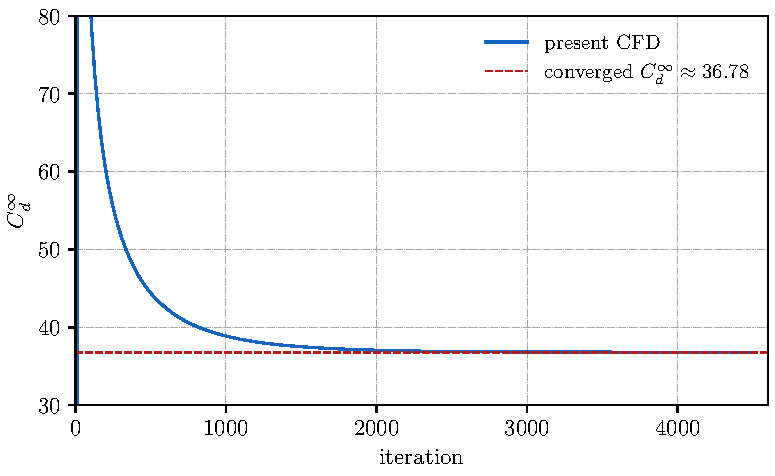
\includegraphics[width=\linewidth]{leaflet_dragCalib_topview.pdf}
  \caption{}
\end{subfigure}\hfill
\begin{subfigure}[b]{0.48\textwidth}
  \centering
  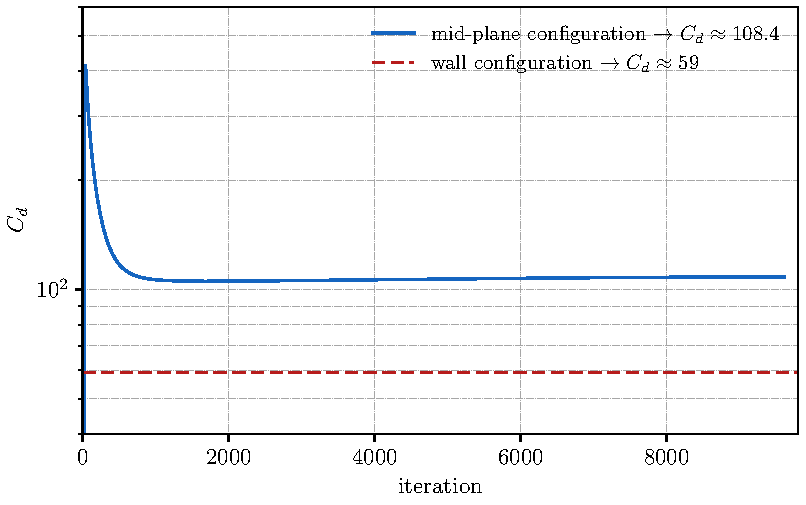
\includegraphics[width=\linewidth]{leaflet_dragCalib_sideview.pdf}
  \caption{}
\end{subfigure}
\caption{Convergence of the two steady-CFD drag calibrations. (a) Free-stream drag coefficient for the unbounded cross-section at $\mathrm{Re}_{t} = 0.212$, converging to $36.8$. (b) In-channel drag coefficient at $\mathrm{Re} = 10$ for the mid-plane configuration (solid, $C_{d} \approx 108$); the horizontal dashed line marks the wall configuration discussed in the text ($C_{d} \approx 59$), in which the leaflet root is clamped to a no-slip wall instead of the channel mid-plane.}
\label{fig:leaflet_dragCalib}
\end{figure}

The dashed line in Figure~\ref{fig:leaflet_dragCalib}(b) marks the value returned by the same case with the two boundary conditions swapped, so that a no-slip wall carries the leaflet root and the opposite side is a symmetry plane. This wall configuration looks plausible at first sight, because it produces a rooted plate with a free upper boundary that resembles a half-channel, but its mirror image is a pair of plates attached to the walls of a full channel with a free gap in the middle, which is not the reference geometry. It returns $C_{d} \approx 59$, roughly half the mid-plane value, because the no-slip boundary layer at the root reduces the local velocity and the smaller effective blockage reduces the pressure rise on the upstream face. The wall configuration therefore returns a wrong but plausible answer for a problem that is visually similar to the coupled geometry, and the only safeguard is the explicit side-by-side comparison shown in the figure. The same diagnostic is recommended for any calibration of this kind in a confined channel. The value passed to the closure is the mid-plane in-channel coefficient at the matching Reynolds number, identified with the closure input through $C_{dn} = C_{d}$, and the tangential coefficient is fixed at $C_{dt} = 0.01$ as before.

\subsection{Upstream-sampling correction and the identification $C_{dn} = C_{d}$}
\label{sec:leaflet_probe}

Identifying $C_{dn}$ with $C_{d}$ is not automatic, because the two are normalised by different velocities. At each beam node the closure samples the local fluid velocity $U_{s}$ at the fixed offset $r_{s} = 3.18\times10^{-3}~\mathrm{m}$ upstream of the node and applies a normal load per unit length of $\tfrac{1}{2}\rho\,C_{dn}\,t_{\ell}\,U_{s}^{2}$, whereas the steady CFD normalises the integrated rigid-plate drag by the channel inlet velocity, giving an equivalent force per unit length of $\tfrac{1}{2}\rho\,C_{d}\,t_{\ell}\,U_{\mathrm{in}}^{2}$ averaged over the plate length. Requiring the two to apply the same force per unit length on average along the beam, so that the calibration carries unchanged into the coupled run, gives
\begin{equation}
\label{eq:cdn_correction}
C_{dn} \;=\; C_{d}\,
\frac{U_{\mathrm{in}}^{2}}{\langle U_{s}^{2}\rangle_{\mathrm{beam}}},
\qquad
\langle U_{s}^{2}\rangle_{\mathrm{beam}} \;\equiv\; \frac{1}{\lambda}\int_{0}^{\lambda} U_{s}^{2}(y)\,\mathrm{d}y,
\end{equation}
so the identification is exact if and only if the beam-averaged squared sampled velocity equals the inlet squared velocity.

To check the condition, a third steady CFD is run on the converged $\mathrm{Re} = 10$ mid-plane configuration, with a sampling line added at $x = L/2 - r_{s}$ and the streamwise velocity extracted at $81$ uniformly spaced points spanning the beam. Squaring the profile and applying Eq.~\eqref{eq:cdn_correction} gives $\langle U_{s}^{2}\rangle_{\mathrm{beam}}/U_{\mathrm{in}}^{2} = 1.006$. Figure~\ref{fig:leaflet_probe_profile} shows why. The curve varies strongly along the beam, reduced to $0.24$ at the root where the plate stagnation slows the flow and rising to $3.36$ at the tip where the fluid accelerates through the narrow gap to the opposite wall, but the two departures balance almost exactly, so the average sits within $0.6\%$ of the reference and the correction can be dropped.

\begin{figure}[!ht]
\centering
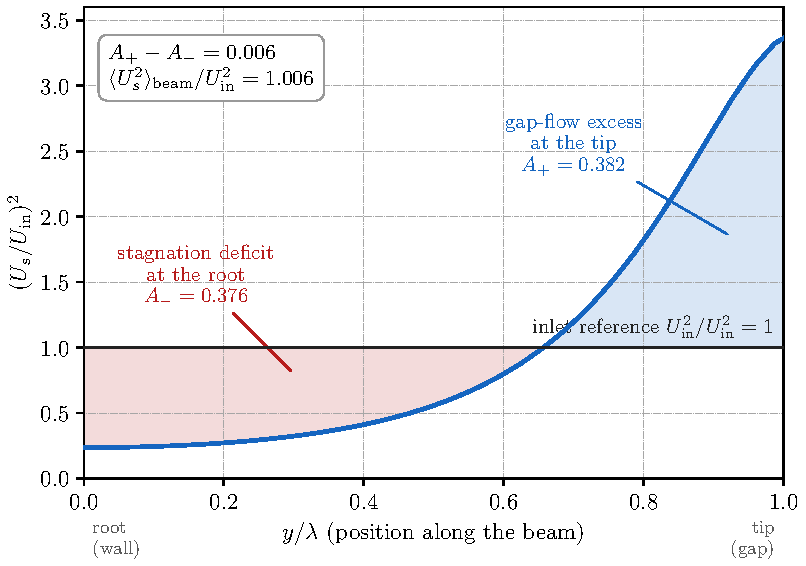
\includegraphics[width=0.72\textwidth]{leaflet_probe_profile.pdf}
\caption{Squared sampled velocity $(U_{s}/U_{\mathrm{in}})^{2}$ along the beam at the upstream-sampling line, in the converged $\mathrm{Re} = 10$ mid-plane field. For $C_{dn} = C_{d}$ to hold exactly, the beam average must equal the inlet reference (horizontal line). The deficit area below the reference near the root ($A_- = 0.376$) is cancelled almost exactly by the excess above it near the tip ($A_+ = 0.382$), leaving the beam average at $1.006$.}
\label{fig:leaflet_probe_profile}
\end{figure}

That the two nearly cancel is specific to this geometry. Without the plate, the sampling line would lie in the undisturbed fully developed channel flow, whose Poiseuille profile peaks at $1.5\,U_{\mathrm{in}}$ on the symmetry plane and integrates to $1.474$, so a leaflet in undisturbed flow would see a $47\%$ enhancement of the squared driving velocity and the correction could not be dropped. The actual plate is a strong blocker, covering $80\%$ of the channel half-width, so most of the upstream flow is forced to stagnate near the root or accelerate through the tip gap and the squared profile is redistributed sharply away from the parabolic shape. In a less confined channel the same probe-line analysis would return a value distinctly above unity, and the explicit correction would have to be retained.

\subsection{Time step and flow snapshots}
\label{sec:leaflet_snapshots}

The temporal resolution is selected from a study on case C1, in which four time steps spanning a factor of twenty are run to statistical convergence with all other inputs held fixed (Figure~\ref{fig:leaflet_dt_study}). The two finest steps collapse onto a common trace, with half-amplitudes of $2.324~\mathrm{mm}$ at $\Delta t = 5\times10^{-5}~\mathrm{s}$ and $2.355~\mathrm{mm}$ at $10^{-4}~\mathrm{s}$, a difference of $1.3\%$ and no visible phase drift over the two reported periods. The two coarser steps under-predict the response, giving $2.036~\mathrm{mm}$ at $2.5\times10^{-4}~\mathrm{s}$ and $2.084~\mathrm{mm}$ at $10^{-3}~\mathrm{s}$. Their non-monotonic ordering indicates that beyond about $2.5\times10^{-4}~\mathrm{s}$ the explicit sampling and quasi-steady closure are no longer integrated with sufficient resolution to track the half-cycle build-up of tip excursion. The finest setting is adopted for all four cases, so that the same step is shared by the higher-$\mathrm{KC}$ cases C3 and C4 without further verification.

\begin{figure}[!ht]
\centering
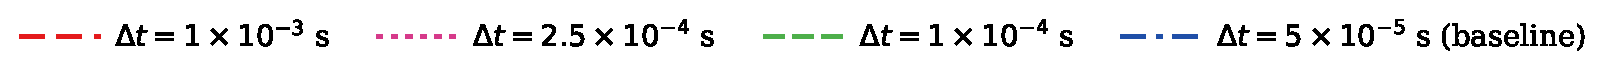
\includegraphics[width=0.90\textwidth]{leaflet_dtStudyLegend.pdf}\\[0.3em]
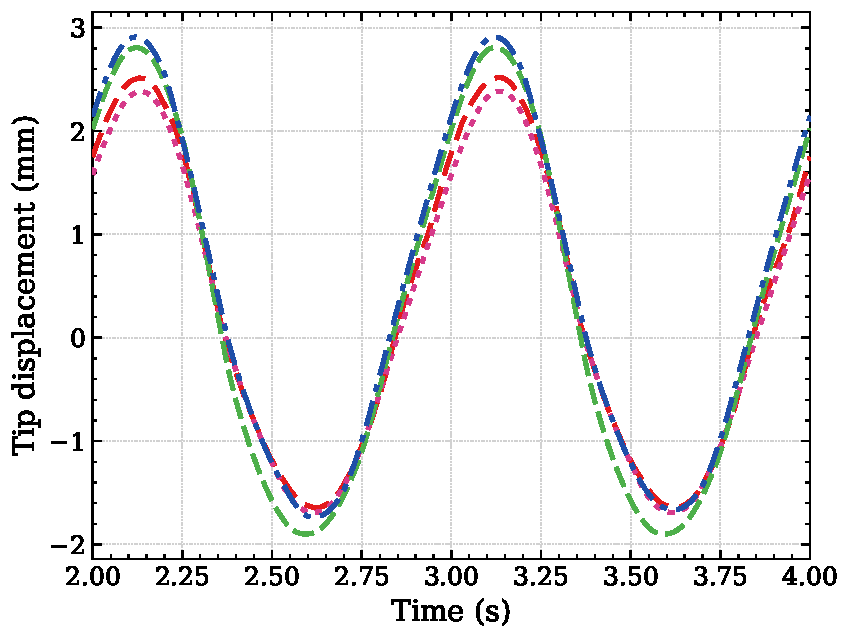
\includegraphics[width=0.68\textwidth]{leaflet_dtStudy.pdf}
\caption{Time-step convergence of the leaflet tip horizontal displacement for case C1 ($\mathrm{Re} = 10$, $\mathrm{St} = 1$), over the converged window $t \in [2, 4]~\mathrm{s}$, with $\Delta t = 5\times10^{-5}~\mathrm{s}$ taken as the converged reference.}
\label{fig:leaflet_dt_study}
\end{figure}

Figure~\ref{fig:leaflet_snapshots_panel} shows the converged field over the first half of a forcing period of case C1, at intervals of $T/8$, with the in-plane streamlines coloured by kinematic pressure and the deflected actuator line overlaid in red. The second half of the period is the mirror image of the first and is not reproduced. Because the imposed inlet signal of Eq.~\eqref{eq:leaflet_inlet} carries a $+\pi/2$ phase shift, the velocity extrema fall at $t = 0$ and $T/2$ and the zero crossings at $T/4$ and $3T/4$. At $t = 0$ the inlet is at peak amplitude, the leaflet attains its instantaneous maximum tip excursion, and a clear pressure dipole develops across the line, with a stagnation patch on the upstream face and a suction patch on the downstream face that switch sides at the opposite extremum. At $T/4$ the inlet velocity crosses zero, the streamlines straighten out as the bulk flow reverses, and the pressure field is comparatively uniform. The small recirculation pair that lingers near the deflected leaflet at that phase is the residual of the previous half-cycle wake, which confirms that the quasi-steady closure does not generate a wake of its own, only the redistribution of the resolved field around the moving line of momentum sinks.

\begin{figure}[!ht]
\centering
\begin{subfigure}[b]{0.48\textwidth}
\centering
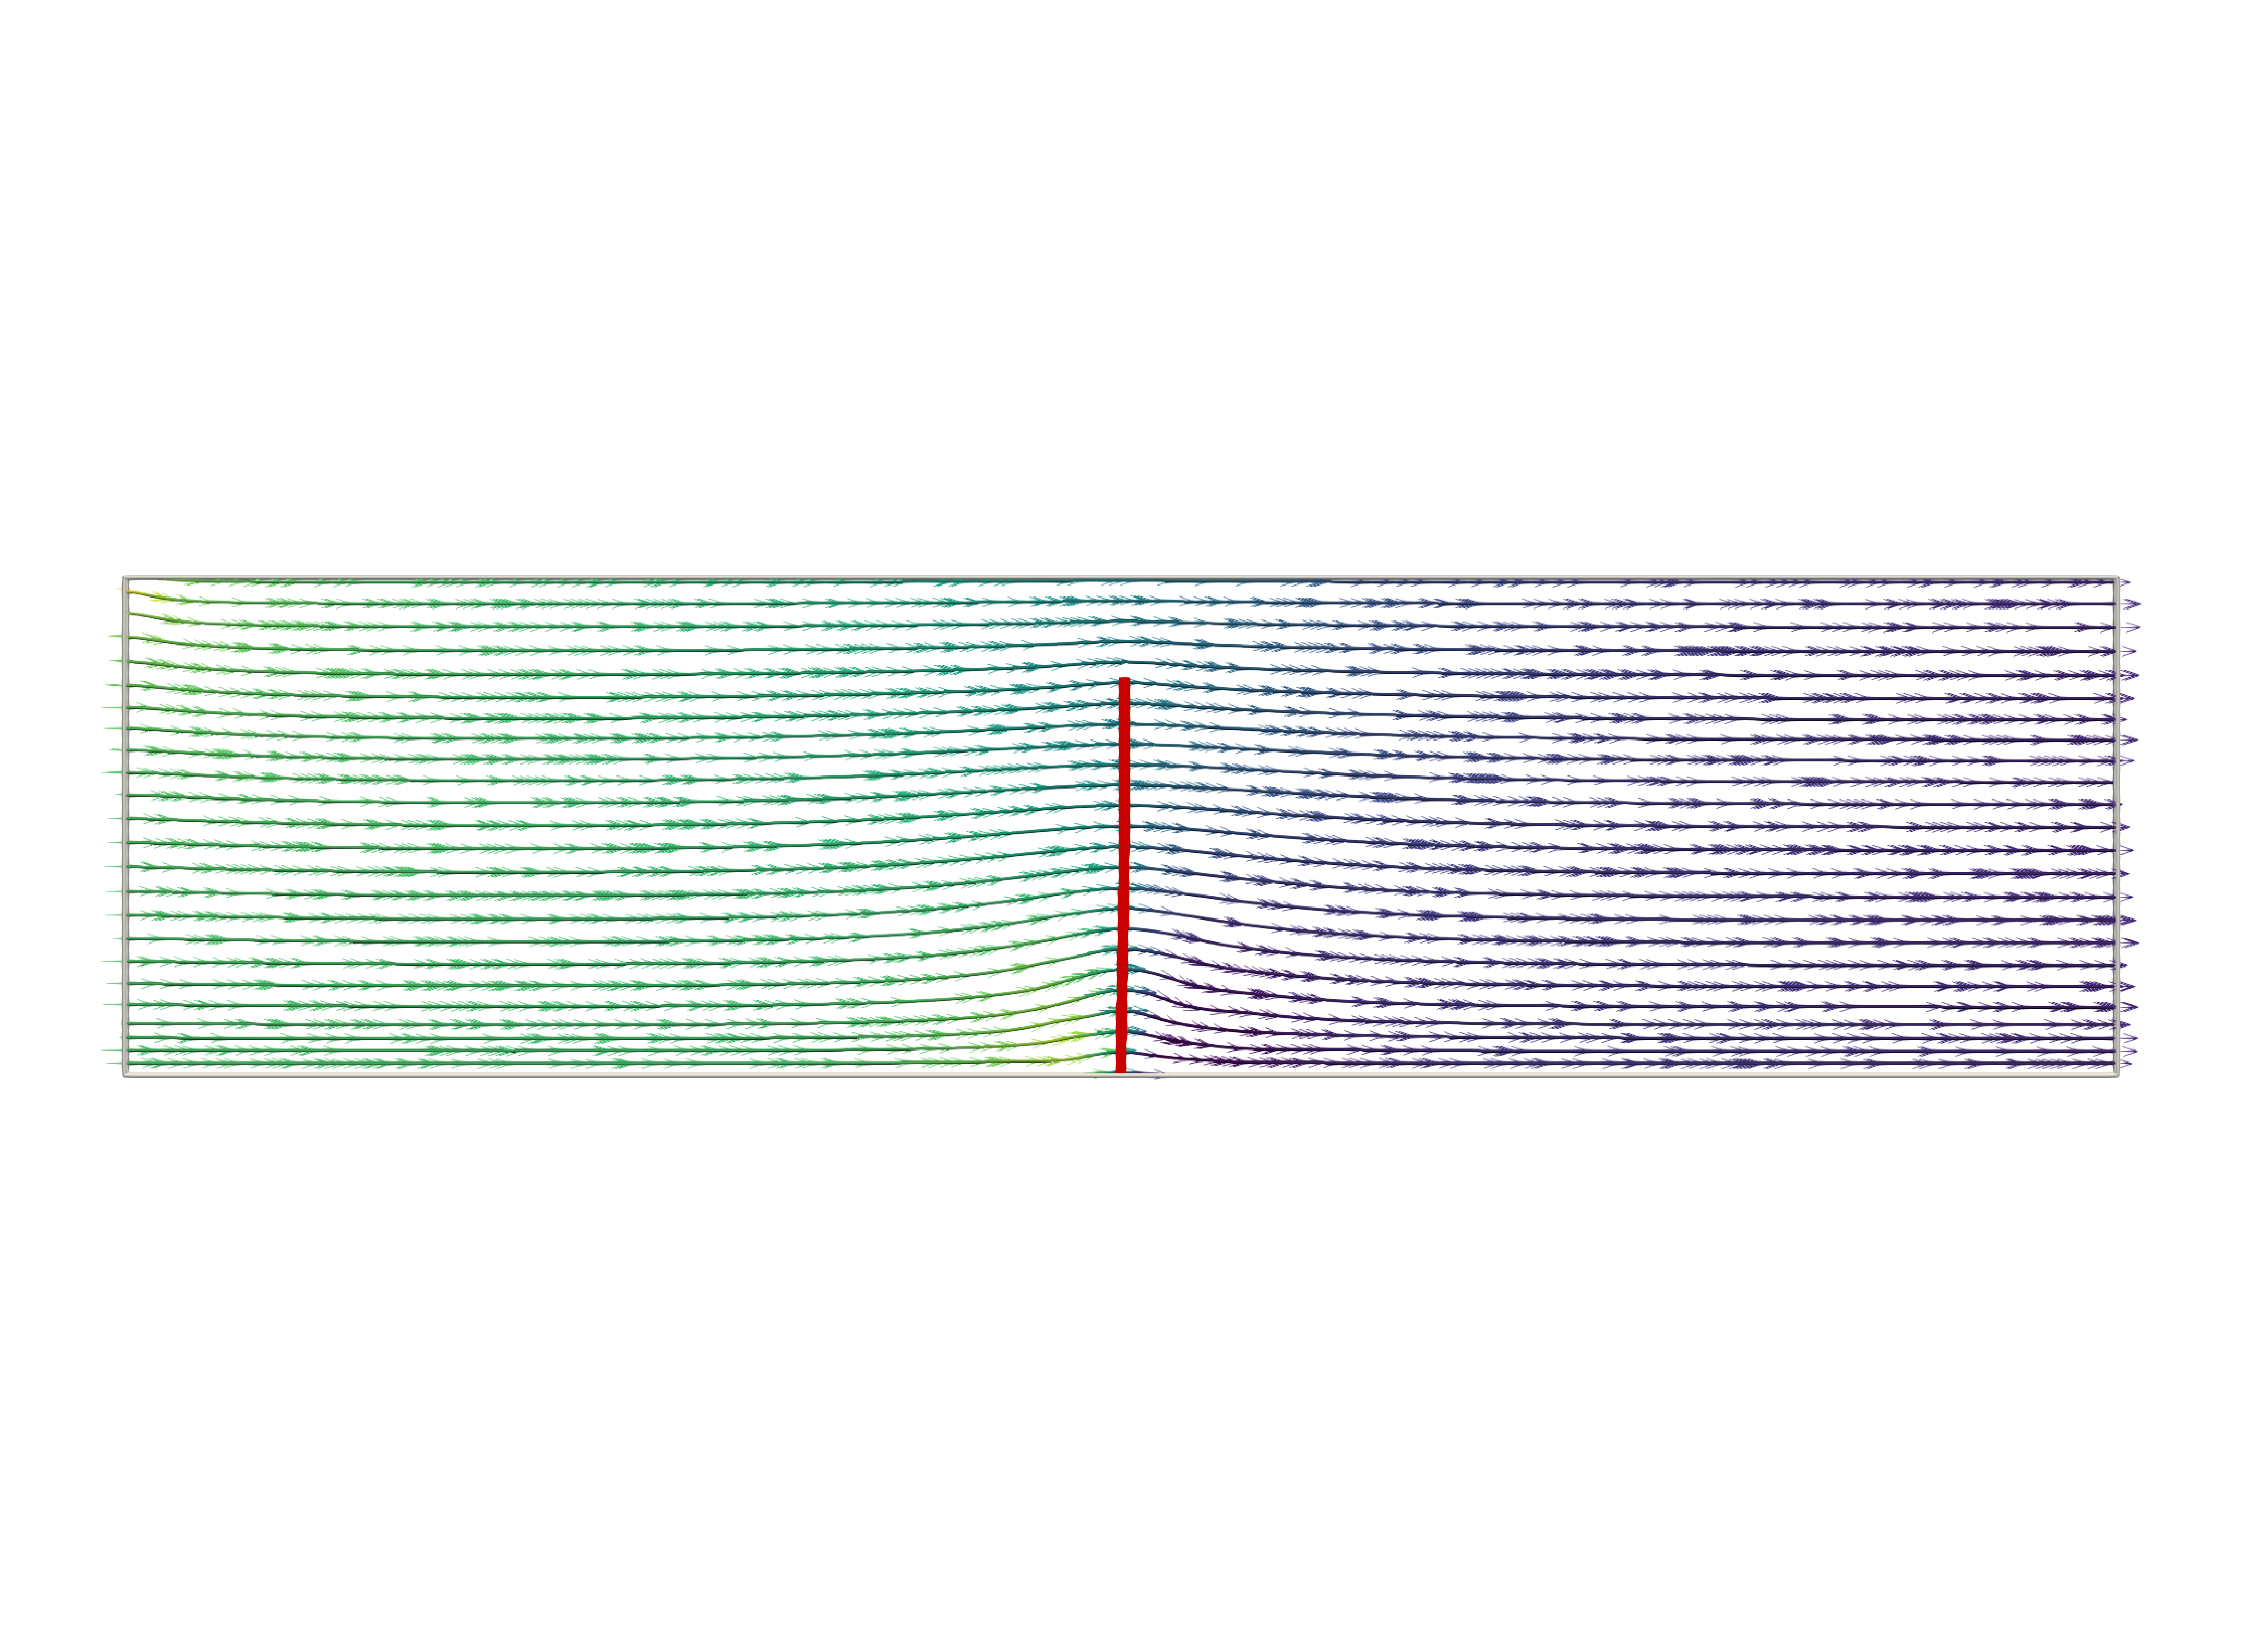
\includegraphics[width=\textwidth]{leaflet_snapshot_t0.pdf}
\caption{$t = 0$}
\end{subfigure}\hfill
\begin{subfigure}[b]{0.48\textwidth}
\centering
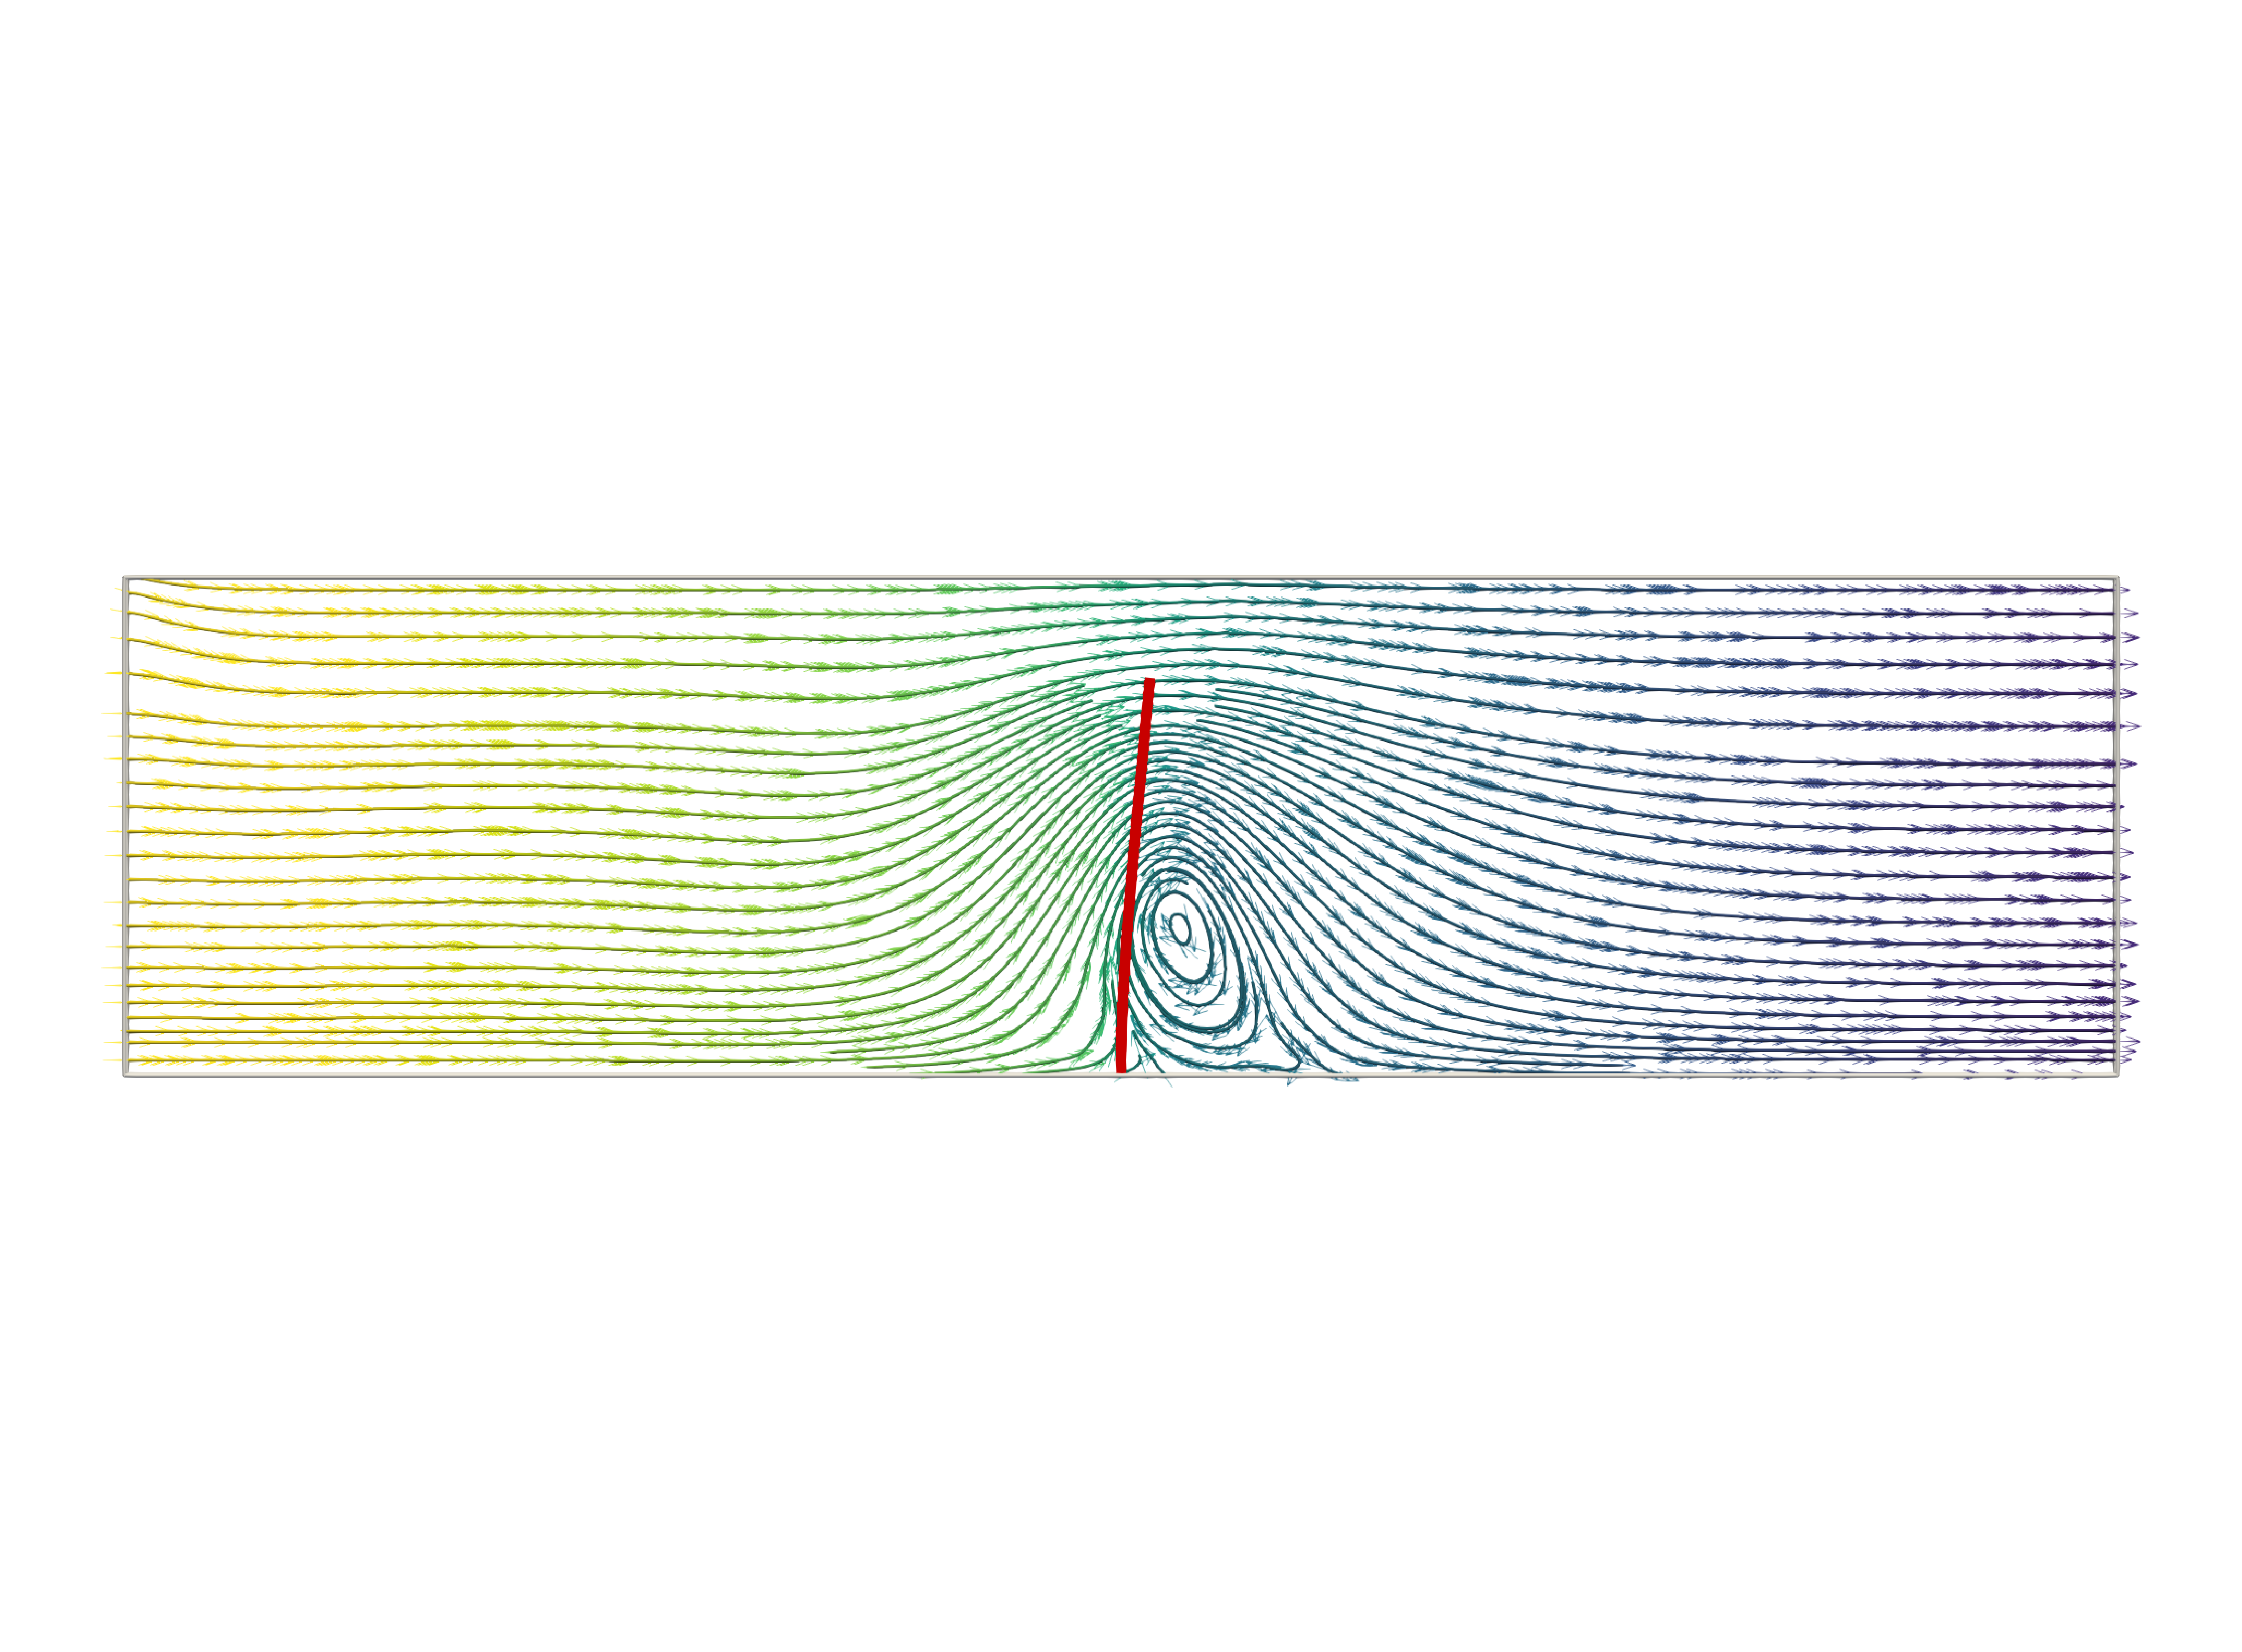
\includegraphics[width=\textwidth]{leaflet_snapshot_t1.pdf}
\caption{$t = T/8$}
\end{subfigure}\\[0.4em]
\begin{subfigure}[b]{0.48\textwidth}
\centering
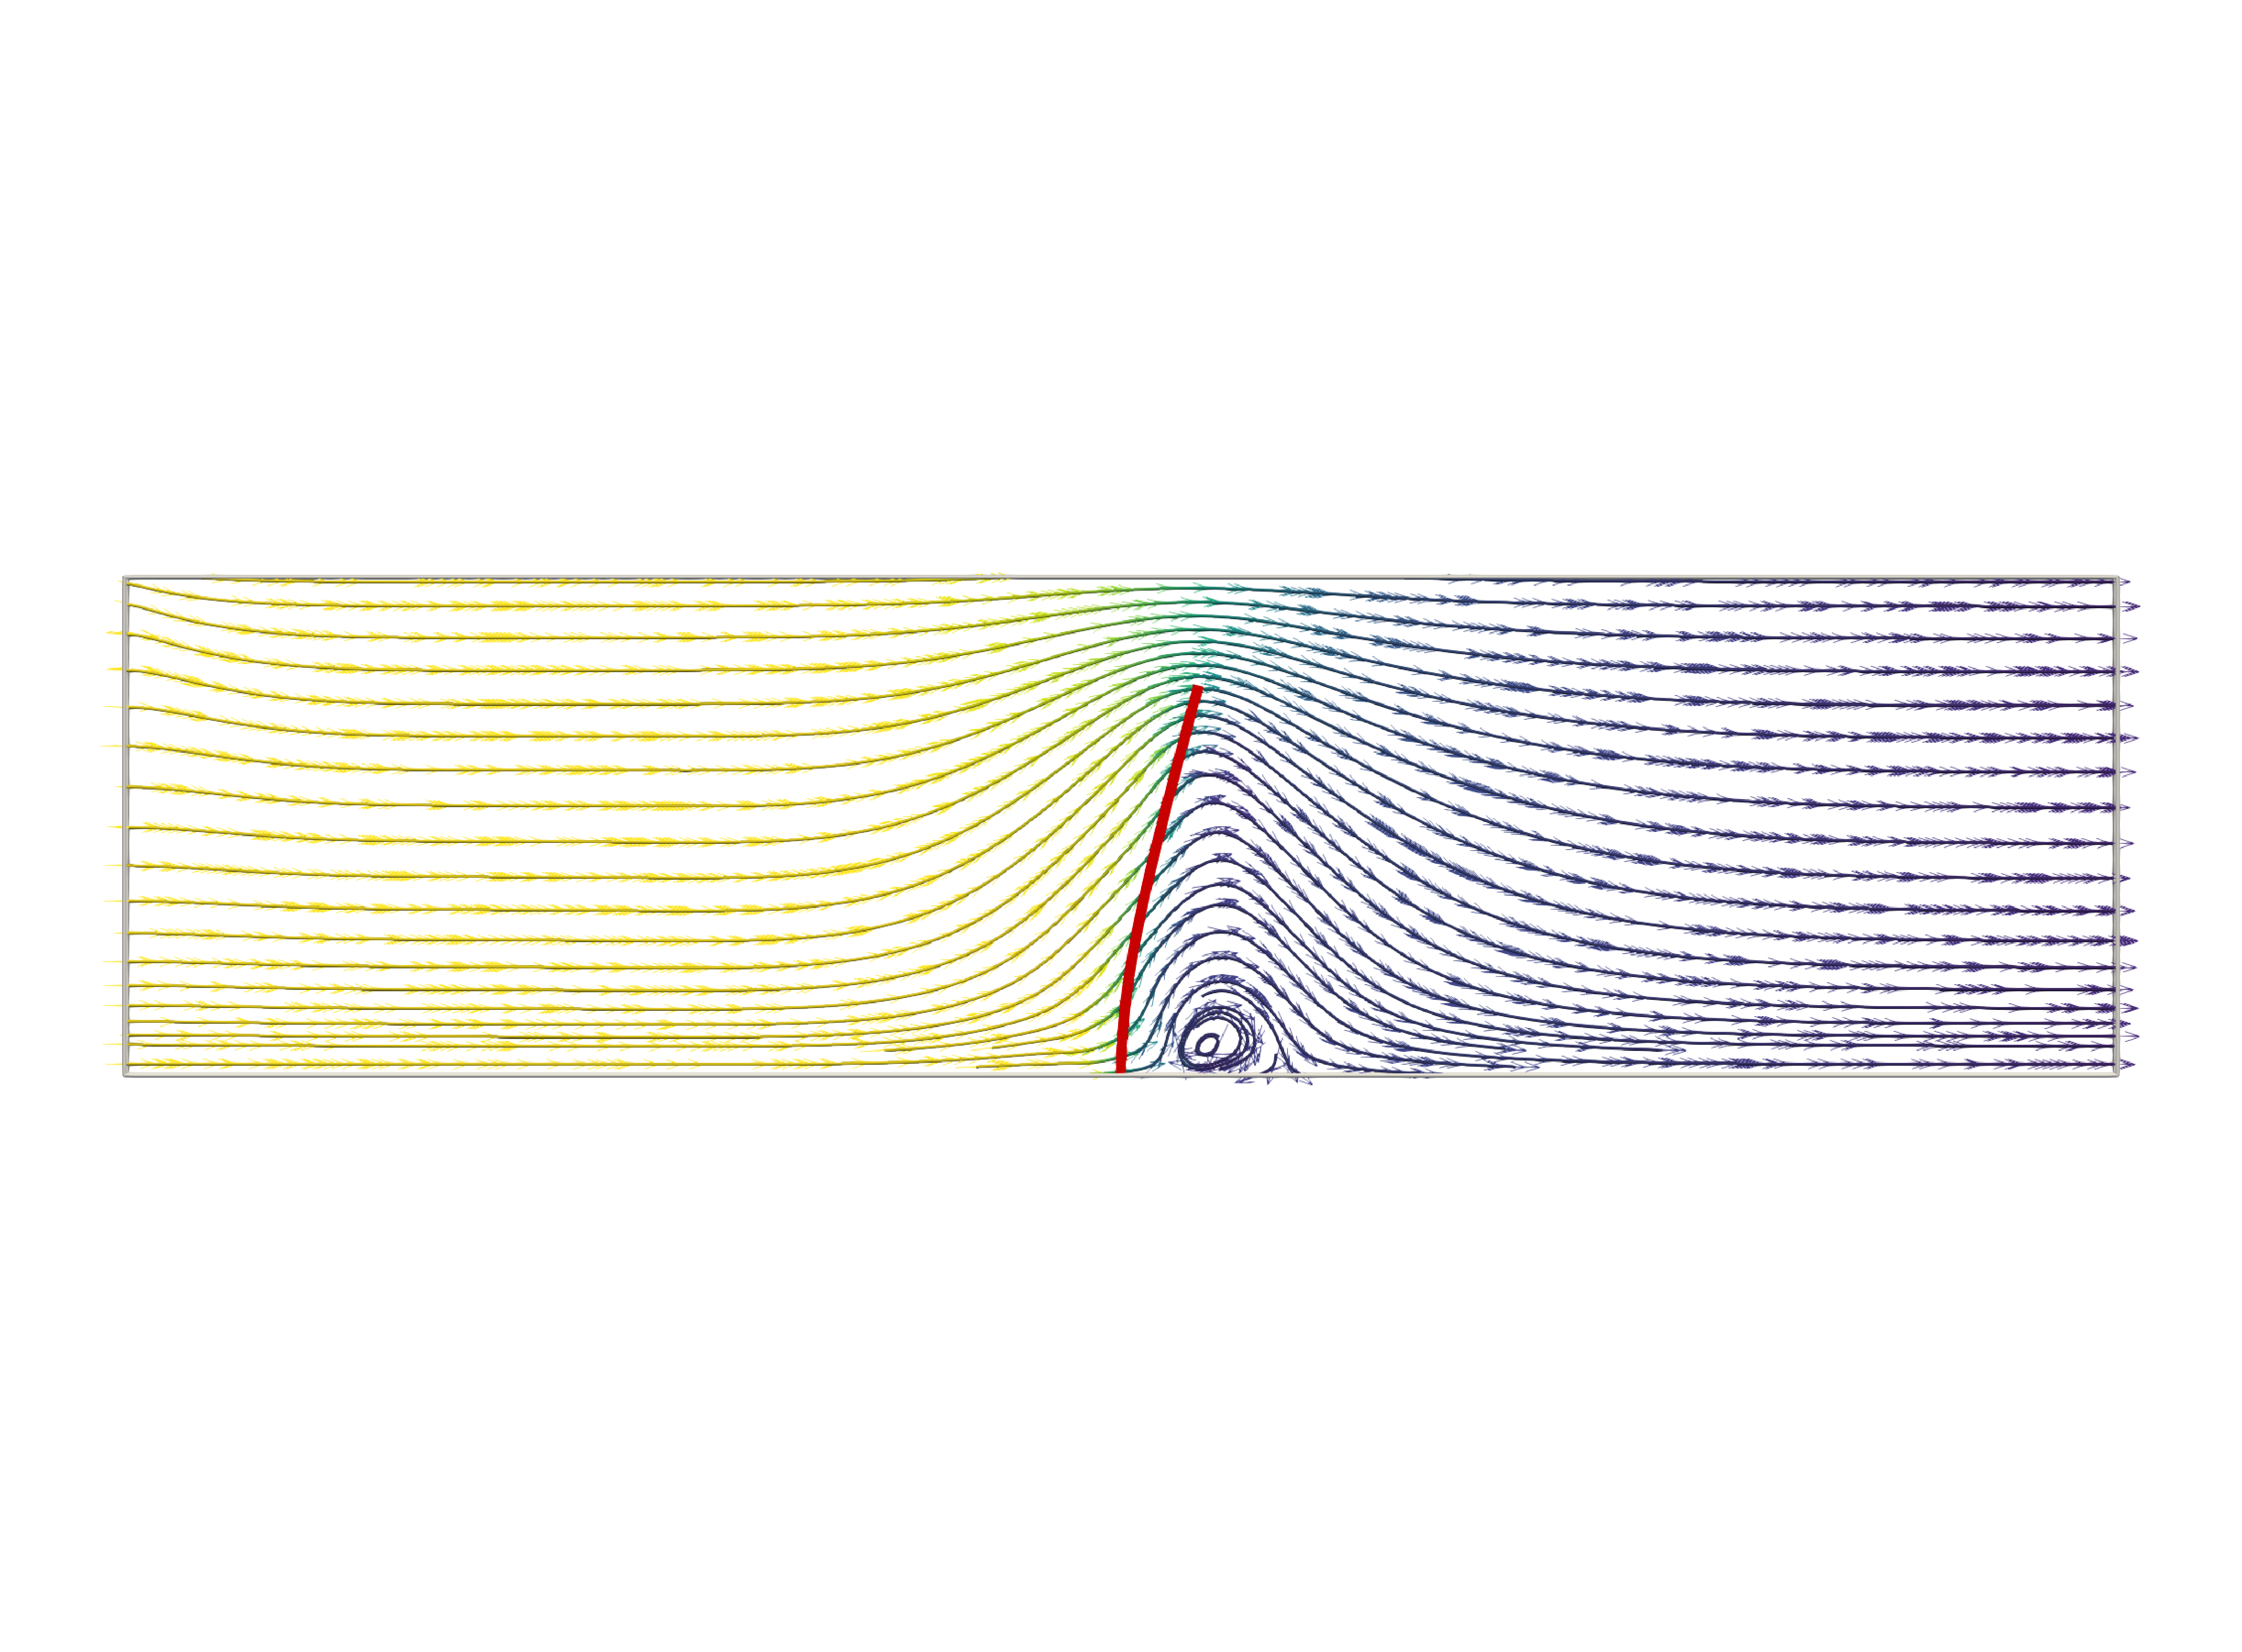
\includegraphics[width=\textwidth]{leaflet_snapshot_t2.pdf}
\caption{$t = T/4$}
\end{subfigure}\hfill
\begin{subfigure}[b]{0.48\textwidth}
\centering
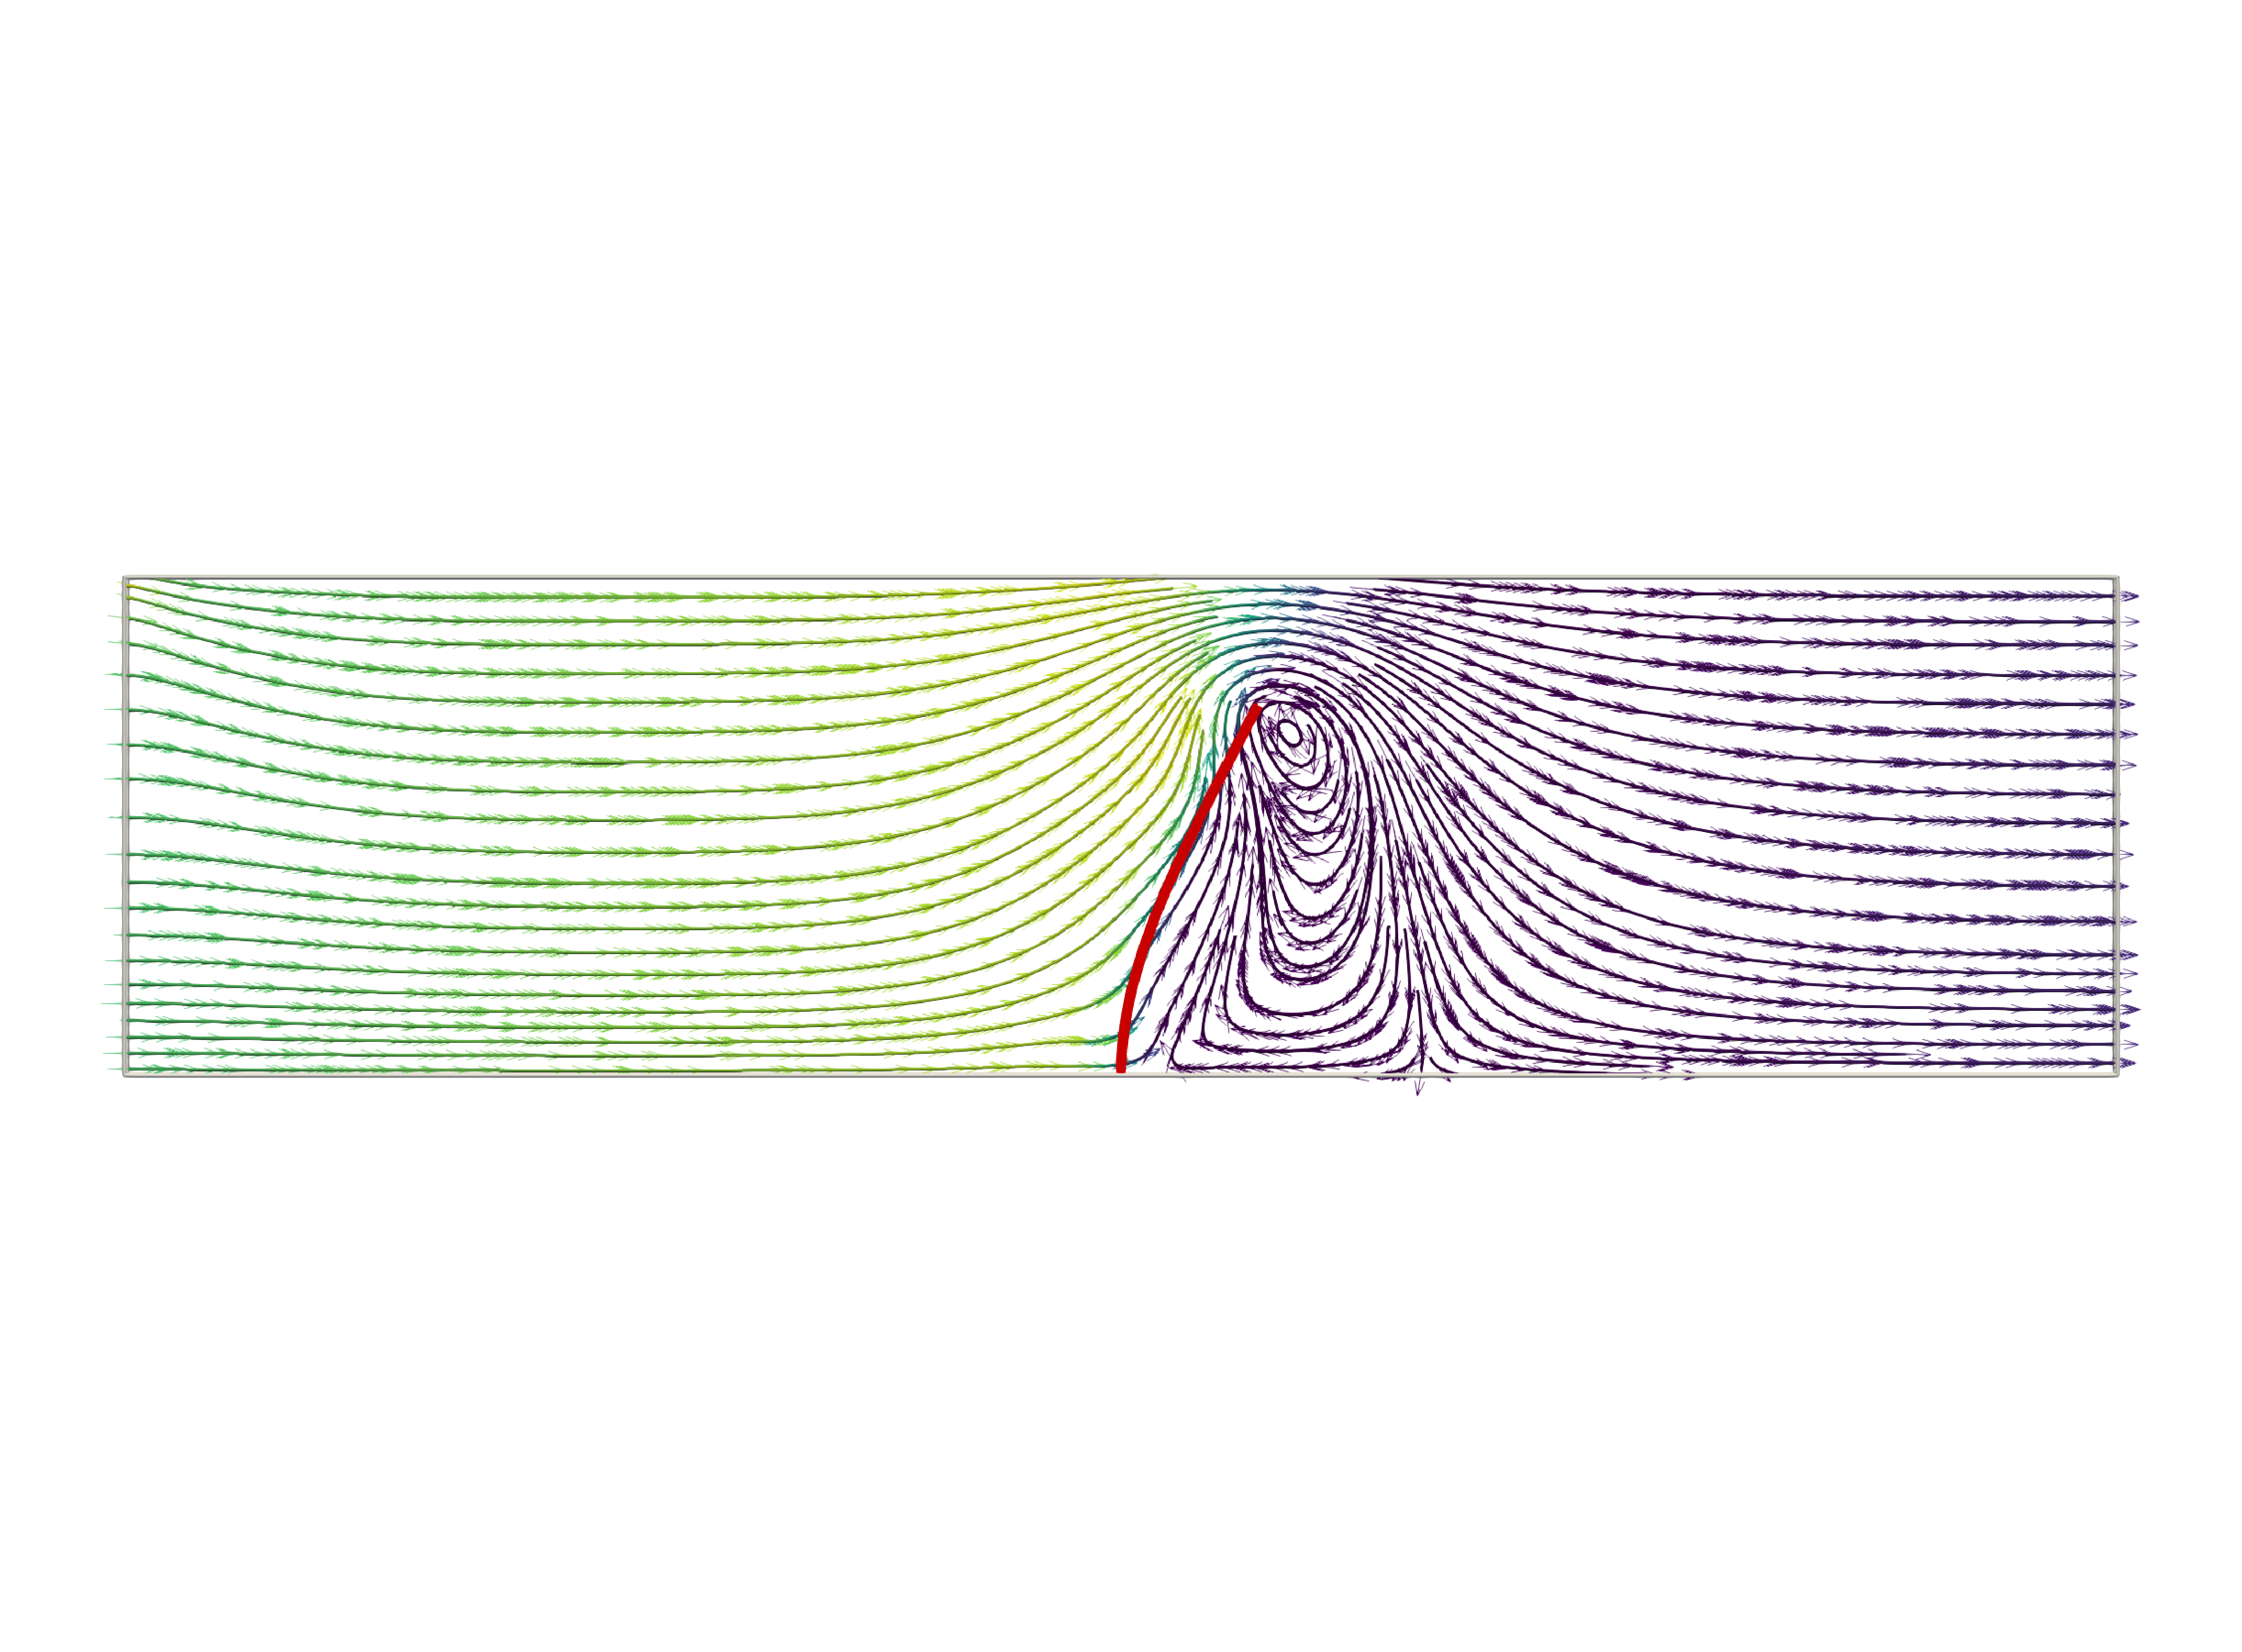
\includegraphics[width=\textwidth]{leaflet_snapshot_t3.pdf}
\caption{$t = 3T/8$}
\end{subfigure}\\[0.4em]
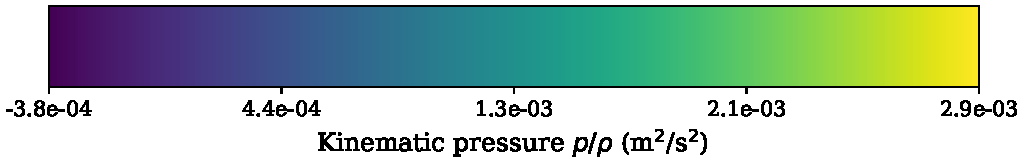
\includegraphics[width=0.80\textwidth]{leaflet_snapshots_cbar.pdf}
\caption{Mid-plane streamlines around the leaflet, coloured by kinematic pressure $p/\rho$ (shared colour bar below), over the first half of a converged forcing period of case C1 ($\mathrm{Re} = 10$, $\mathrm{St} = 1$, $T = 1~\mathrm{s}$), with the deflected actuator line overlaid in red. The second half of the period mirrors the first.}
\label{fig:leaflet_snapshots_panel}
\end{figure}

Three features connect to the results below. The absence of any small-scale vortex shedding throughout the period is consistent with the low cross-section Reynolds number of case C1 and supports the use of a $\mathrm{KC}$-independent drag coefficient. The tip excursion in the peak frame is visually consistent with the $\pm 2.324~\mathrm{mm}$ half-amplitude reported below, which provides a field-level check on the integral trace. The pressure dipole is generated entirely by the projected body force back-reacting on the fluid, so although the leaflet is geometrically absent from the mesh, its presence in the momentum equation produces a qualitatively analogous upstream-stagnation and downstream-suction structure to what a body-fitted simulation would resolve at the plate surface, with the redistribution length set by the kernel width rather than by the plate thickness.

\subsection{Verification across the four (Re, St) cases}
\label{sec:leaflet_results}

The coupled simulation is run at the four combinations of Table~\ref{tab:leaflet_cases}. All four runs share the same beam discretisation, fluid mesh, kernel width, and time step, and only the inlet amplitude, the forcing period, and the matching $C_{dn}$ vary. The reference traces are digitised from Figs.~13 and 14 of the reference paper.

\begin{figure}[!ht]
\centering
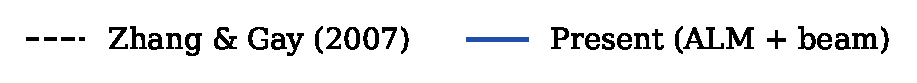
\includegraphics[width=0.90\textwidth]{leaflet_panel_legend.pdf}\\[0.3em]
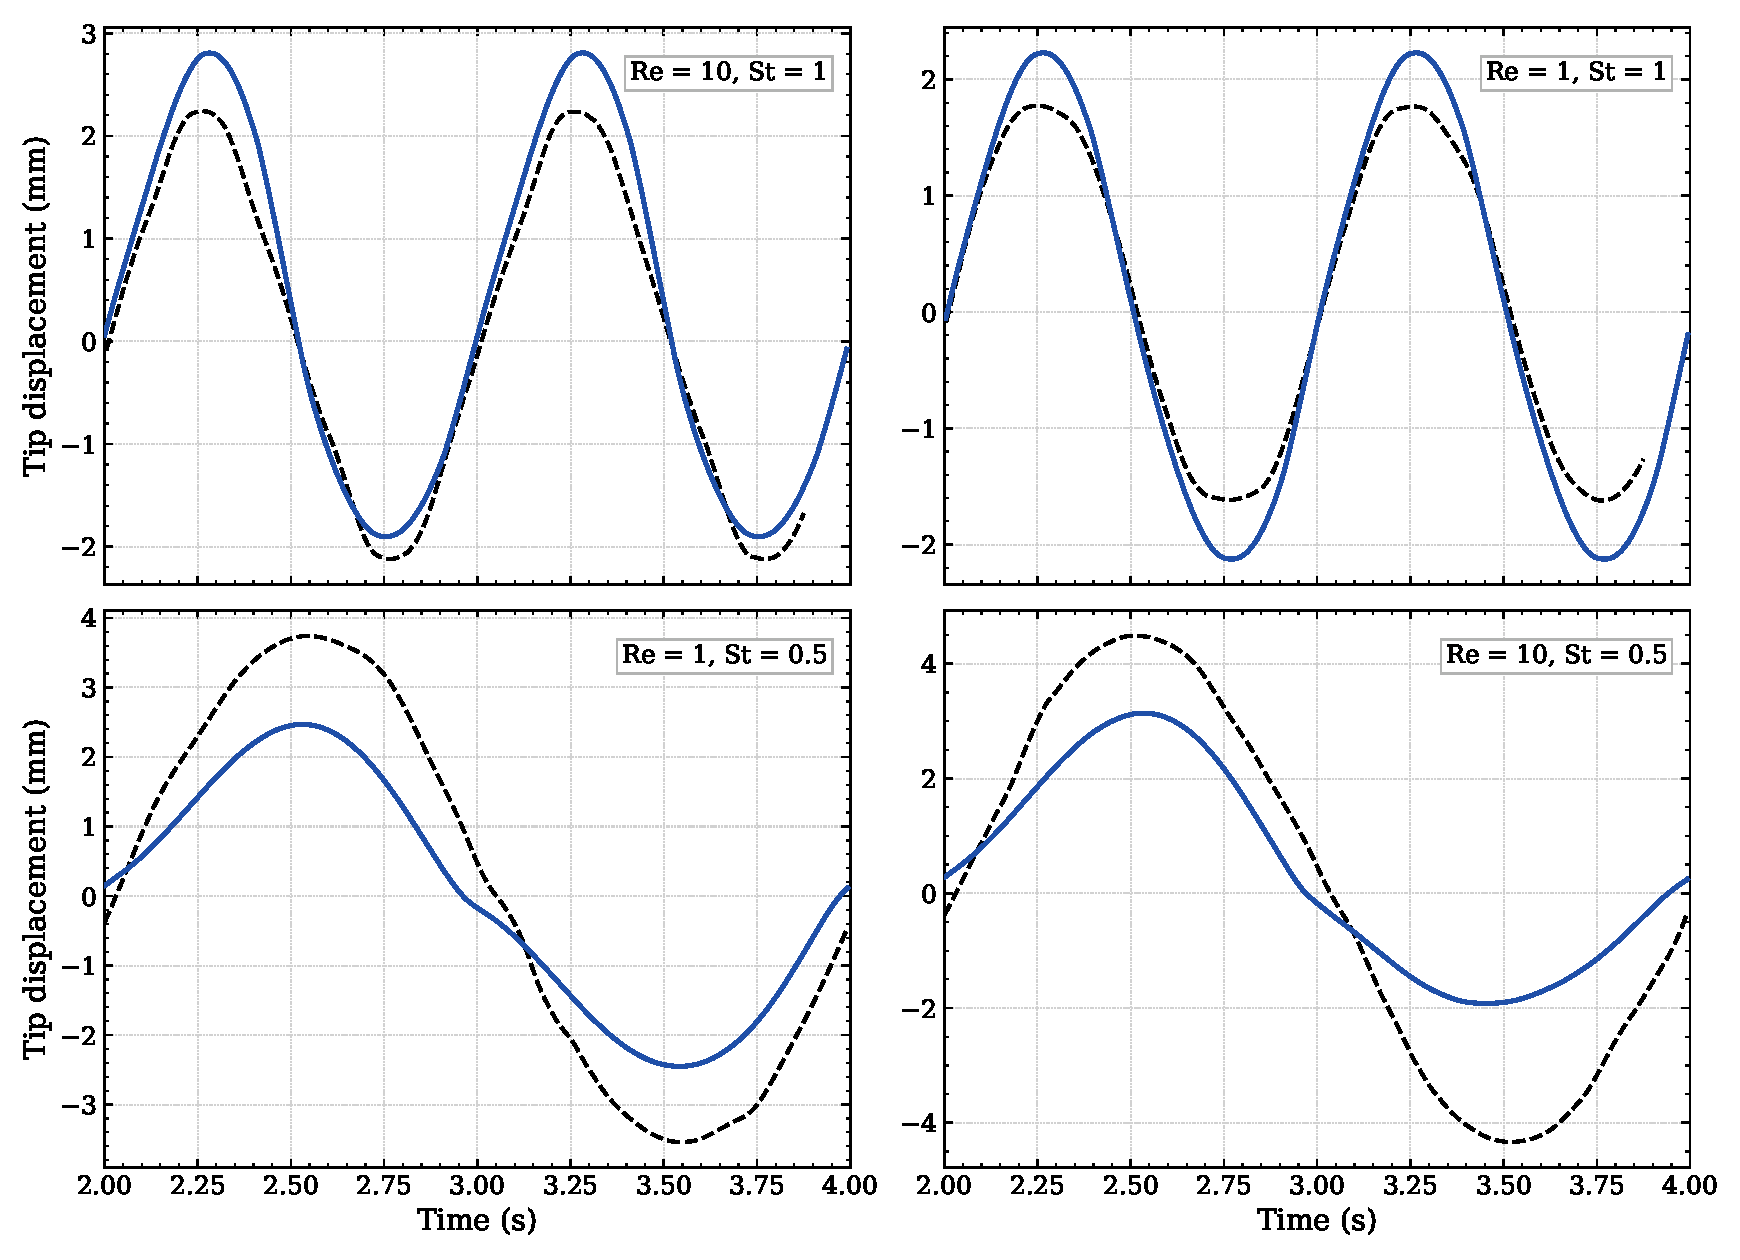
\includegraphics[width=\textwidth]{leaflet_panel.pdf}
\caption{Tip horizontal displacement traces for the four (Re, St) cases of \citet{zhang_immersed_2007}, Section~3.2. Dashed black lines are the digitised reference traces and solid blue lines the present result. Each trace has been phase-aligned to the reference by cross-correlation and windowed to the converged interval $t \in [2, 4]~\mathrm{s}$.}
\label{fig:leaflet_results_4cases}
\end{figure}

Figure~\ref{fig:leaflet_results_4cases} compares the simulated tip displacement against the reference over the converged window. The agreement falls into two families. The cases at $\mathrm{St} = 1$ (C1 and C2) reproduce the reference period exactly and overshoot its peak excursion, the present values being $\pm 2.324~\mathrm{mm}$ against $\pm 2.2~\mathrm{mm}$ at C1 and $\pm 2.2~\mathrm{mm}$ against $\pm 1.7~\mathrm{mm}$ at C2, with the phase coinciding within plotting accuracy and the cycle-to-cycle shape closely matched. The cases at $\mathrm{St} = 0.5$ (C3 and C4) behave differently. The simulated peak excursion is essentially fixed near $\pm 2.5~\mathrm{mm}$, whereas the reference reaches $\pm 3.7~\mathrm{mm}$ at C3 and $\pm 4.5~\mathrm{mm}$ at C4, so the simulation under-predicts by about one third at C3 and by more than $40\%$ at C4. The period is again reproduced exactly, so the discrepancy is purely in amplitude.

\AUTHORNOTE{%
\textbf{Two numbers in this paragraph disagree with the analysis output and need checking
against the run data.} The thesis text this paragraph is based on reported the C2 pair as
$\pm 2.2~\mathrm{mm}$ simulated against $\pm 1.7~\mathrm{mm}$ measured, whereas the
cross-correlation analysis script that produced Figure~\ref{fig:leaflet_results_4cases}
reported $\pm 1.85$ against $\pm 1.75~\mathrm{mm}$, which is a $6\%$ over-prediction rather
than a $29\%$ one. The two cannot both be right, and which one is correct changes the
headline claim for the $\mathrm{St} = 1$ family from ``within $10\%$ at both Reynolds
numbers'' to ``within $10\%$ at C1 and $29\%$ over at C2''. Please read the C2 half-amplitude
off the run and fix whichever is wrong. Separately, the same thesis paragraph stated the
$\mathrm{St} = 0.5$ deficit as $30\%$ ``in both cases'', which does not follow from the
values printed alongside it, since $2.5$ against $3.7$ is $32\%$ and $2.5$ against $4.5$ is $44\%$.
The sentence above has been corrected to match its own numbers, and the abstract and
conclusions now say ``more than $30\%$'', which holds either way.
}

\paragraph{Origin of the Strouhal-dependent discrepancy.}
The quasi-steady closure of Eq.~\eqref{eq:almLineForce} depends only on the instantaneous sampled velocity, and carries no fluid-inertia term proportional to the acceleration. In the IFEM reference the leaflet is immersed in a fully resolved Navier--Stokes field, so its force balance includes an added-mass term scaling with the local fluid acceleration and a history term depending on the past evolution of the relative motion. Halving the Strouhal number doubles the forcing period and halves the peak fluid acceleration at the inlet, and for a stationary member in an oscillating stream the classical Morison scaling would then predict the \emph{opposite} of the observed trend, since the ratio of inertia to drag scales as $1/\mathrm{KC}$ \citep{sarpkaya_mechanics_1981}. The growing under-prediction at $\mathrm{St} = 0.5$ must therefore originate in the unsteady forces associated with the leaflet's own motion, which the fixed-body scaling does not describe. At the longer period the reference excursion roughly doubles, so the relative acceleration between the leaflet and the surrounding fluid, and with it the added-mass reaction on the moving structure, remains dynamically significant even as the inlet acceleration halves, while at $\mathrm{Re}_{t} \approx 0.2$ the viscous history contribution depends on the past relative motion in a way that no instantaneous coefficient can represent. A direct force decomposition of the reference solution would be required to apportion the deficit among these terms, and it is not available from the published data, so what the present results establish is the operational boundary of the closure rather than the split between the missing terms.

One further observation supports this picture. The drag coefficient of the rigid plate is essentially independent of the Keulegan--Carpenter number in this regime, an unsteady re-run of the rigid-plate calibration at $\mathrm{KC} = 47$ and $94$ giving $C_{d} \approx 107$ in both. The textbook $C_{dn}(\mathrm{KC})$ trend that operates at higher Reynolds numbers does not apply at $\mathrm{Re}_{t} \approx 0.2$, where the wake remains attached and vortex shedding is suppressed. The Strouhal-dependent discrepancy is therefore not driven by a Strouhal-dependent drag coefficient on the rigid plate. It is driven by the unsteady inertia of the surrounding fluid acting on the moving leaflet, which is precisely the term that the classical Morison equation separates from the quadratic drag and that the present closure does not carry.

The deterioration is documented quantitatively here rather than removed by case-specific recalibration. Replacing the steady-CFD $C_{dn}$ with a per-case empirical value would mask the modelling limitation behind a parameter sweep, whereas the present calibration is fixed once by a separate, geometry-only CFD and applied unchanged across the four cases. The framework is therefore verified over a clearly defined range of conditions, namely the drag-dominated regime represented here by the Strouhal number of $1$ rather than $0.5$, and extending it further would require an unsteady closure that adds explicit added-mass and history terms to Eq.~\eqref{eq:almLineForce}.

\AUTHORNOTE{%
\textbf{Optional run that would sharpen this section.} The $\mathrm{St} = 0.5$ deficit is
attributed to unsteady forces on the \emph{moving} leaflet, and the supporting evidence is
indirect (the rigid-plate $C_{d}$ is $\mathrm{KC}$-independent, so the deficit cannot be a
$C_{d}(\mathrm{KC})$ effect). A forced-oscillation \texttt{pimpleFoam} run on the rigid plate
at $\mathrm{St} = 0.5$, with the plate \emph{prescribed} to follow the C4 tip trajectory,
would give the in-phase and out-of-phase force components directly and turn the attribution
into a measurement. It is one short two-dimensional run on the existing calibration case.
Without it, a reviewer may reasonably ask for the decomposition, and the present answer is
that the published data do not permit it.
}
